\documentclass[12pt, letterpaper]{article}

% ==========================================
%              DOCUMENT PACKAGES
% ==========================================

% --- Core Language & Encoding ---
\usepackage[english]{babel} % Sets the language and regional settings for English documents
\usepackage[utf8]{inputenc} % Allows the use of UTF-8 characters in the document
\usepackage[T1]{fontenc} % Specifies the font encoding
\usepackage[margin=2cm]{geometry} % Sets the page margins

% --- Colors & Graphics ---
\usepackage[table,dvipsnames]{xcolor} % Advanced color management
% \usepackage{color} % Basic package for text and background colors
\usepackage{graphicx} % Enhanced support for including external images and scaling them
\usepackage{adjustbox} % Adjusts the size, scaling, and alignment of boxes, images, and tables
% \usepackage{background} % Allows adding background images or watermarks to pages
\usepackage{float} % Improves the interface for floating objects and adds the [H] placement
\usepackage{pdflscape} % Makes landscape pages display correctly on screen in PDF viewers
\usepackage{pdfpages} % Allows the inclusion of external multi-page PDF documents

% --- Math, Science & Engineering ---
\usepackage{amsfonts} % Provides extended mathematical fonts
\usepackage{amsmath} % Provides advanced mathematical typesetting and environments
\usepackage{amssymb} % Provides extended mathematical symbols
% \usepackage{amsmath, amssymb} % (Redundant combination line omitted for stability)
\usepackage{amsthm} % Facilitates the creation of theorem-like environments
\usepackage{mathtools} % Enhances amsmath with additional math tools and bug fixes
\usepackage{thmtools} % Extensions and customization options for theorem environments
\usepackage{nicematrix} % Enhances matrices and tabulars using PGF/TikZ
\usepackage{xy} % Typesets complex graphs and diagrams
\usepackage{circuitikz} % Allows drawing of electrical networks and circuits

% --- Typography & Fonts ---
\usepackage{avant} % Sets the default sans-serif font to Avant Garde
\usepackage{cantarell} % Sets the default sans-serif font to Cantarell
\usepackage{charter} % Sets the default roman font to Charter
\usepackage{cmbright} % Sets the font family to Computer Modern Bright 
\usepackage{helvet} % Sets the default sans-serif font to Helvetica
\usepackage{inconsolata} % Sets the default typewriter (monospace) font to Inconsolata
\usepackage{iwona} % Sets the font family to Iwona 
\usepackage{kurier} % Sets the font family to Kurier 
\usepackage{lmodern} % Loads the Latin Modern fonts 
\usepackage{textcomp} % Provides additional text symbols
\usepackage{ulem} % Provides various types of text underlining and strikethroughs

% --- Tables & Lists ---
\usepackage{array} % Extends the array and tabular environments
\usepackage{arydshln} % Allows dashed lines in arrays and tables
\usepackage{bigstrut} % Adds custom vertical space in table rows
\usepackage{booktabs} % Enhances the quality of tables with better horizontal rules
% \usepackage{colortbl} % Allows coloring of rows, columns, and individual cells in tables
\usepackage{diagbox} % Creates table cells with diagonal lines 
\usepackage{enumitem} % Provides advanced control over list environments
\usepackage{longtable} % Allows tables to break across multiple pages
\usepackage{multirow} % Allows individual table cells to span across multiple rows
\usepackage{tabularx} % Creates tables with dynamically adjustable-width columns
\usepackage{pgfplotstable} % Reads and cleanly formats numerical tables directly from CSV

% --- Formatting, Layout & UI ---
\usepackage{blindtext} % Generates dummy text for testing document layouts
\usepackage{caption} % Customizes captions in floating environments
\usepackage{comment} % Allows you to block out large sections of text
\usepackage{emptypage} % Automatically removes headers and footers on empty pages
\usepackage{fancyhdr} % Allows complete customization of headers and footers
\usepackage{fancyvrb} % Enhanced verbatim environments for writing raw code
\usepackage{framed} % Creates framed, shaded, or differently highlighted text regions
\usepackage{fullpage} % Quickly sets all page margins to 1 inch
\usepackage{lipsum} % Generates Lorem Ipsum dummy text
\usepackage{mdframed} % Creates highly customizable framed environments
\usepackage{multicol} % Allows intermixing single and multiple text columns
\usepackage{parskip} % Replaces standard paragraph indentation with vertical spacing
\usepackage{setspace} % Controls line spacing (single, one-and-a-half, double)
\usepackage{subcaption} % Supports sub-figures and sub-tables with independent captions
% \usepackage{subfig} % Older package for sub-figures (subcaption is generally preferred now)
\usepackage{tcolorbox} % Creates heavily customized colored and framed text boxes
\usepackage{titlesec} % Customizes the formatting of section, subsection, and chapter headings
\usepackage{titling} % Provides advanced control over the typesetting of the document title

% --- Bibliographies & References ---
\usepackage{biblatex} % Advanced, modern bibliographic processing and formatting
\usepackage{csquotes} % Context-sensitive quotation facilities
\usepackage{makeidx} % Supports the generation of a document index
% \usepackage{natbib} % Flexible bibliography support, particularly for author-year citation styles

% --- TikZ & Plotting ---
\usepackage{tikz} % Advanced package for creating vector graphics and diagrams programmatically
\usepackage{pgf-pie} % Draws pie charts programmatically using PGF/TikZ
\usepackage{pgfplots} % Creates high-quality mathematical plots, charts, and graphs
% \usepackage{fancytikzposter} % Used to create large format academic posters using TikZ

% --- URLs & Hyperlinks ---
\usepackage{url} % Formats and properly hyphenates long URLs
\usepackage{breakurl} % Allows line breaks in URLs, especially when compiled with latex -> dvips
\usepackage{hyperref} % Creates cross-referencing, clickable links, and PDF bookmarks

% --- Code Formatting ---
\usepackage{listings} % Typesets programming source code with formatting and syntax highlighting


% ==========================================
%           DOCUMENT CONFIGURATION
% ==========================================

% Custom color definitions
\definecolor{mygray}{gray}{0.9}

% Hyperlink configuration
\hypersetup{
    colorlinks=true,
    linkcolor=blue,
    urlcolor=blue
}

% Configuración adicional para breaks en URLs
\def\UrlBreaks{\do\/\do-\do_\do.\do=\do?\do\&}
\expandafter\def\expandafter\UrlBreaks\expandafter{\UrlBreaks\do\a\do\b\do\c\do\d\do\e\do\f\do\g\do\h\do\i\do\j\do\k\do\l\do\m\do\n\do\o\do\p\do\q\do\r\do\s\do\t\do\u\do\v\do\w\do\x\do\y\do\z}

%Uncomment the following lines to use a sans-serif font
%\usepackage{helvet}
%\renewcommand{\familydefault}{\sfdefault}

% TikZ libraries
\usetikzlibrary{shapes.geometric, positioning, decorations.pathreplacing}

\graphicspath{ {./img/} } % Sets the path for the graphics

\newlist{biblio}{enumerate}{1}
\setlist[biblio,1]{
    label=[\arabic*],
    leftmargin=2.2em,
    labelsep=0.5em,
    itemsep=0.35em,
    parsep=0pt,
    topsep=0.35em,
    align=left
}

\makeindex

% \tiny
% \scriptsize
% \footnotesize
% \small
% \normalsize (default size)
% \large
% \Large
% \LARGE
% \huge
% \Huge


% ==========================================
%         GLOBAL LISTINGS SETTINGS
% ==========================================
\lstset{
	basicstyle=\ttfamily\small,
	numbers=left,
	numberstyle=\tiny\color{gray},
	stepnumber=1,
	numbersep=10pt,
	backgroundcolor=\color{white},
	showspaces=false,
	showstringspaces=false,
	breaklines=true,
	frame=single,
	tabsize=2, 
    captionpos=b, 
    lineskip=-1pt,
	extendedchars=true,
	literate={á}{{\'a}}1 {é}{{\'e}}1 {í}{{\'i}}1 {ó}{{\'o}}1 {ú}{{\'u}}1 {Á}{{\'A}}1 {É}{{\'E}}1 {Í}{{\'I}}1 {Ó}{{\'O}}1 {Ú}{{\'U}}1 {ñ}{{\~n}}1 {Ñ}{{\~N}}1 {¿}{{\textquestiondown}}1 {¡}{{\textexclamdown}}1
}

% ==========================================
%            LANGUAGE: SQL
% ==========================================
\lstdefinestyle{sqlstyle}{
	language=SQL,
	keywordstyle=\color{blue}\bfseries,
	commentstyle=\color[rgb]{0,0.5,0}\itshape,
	stringstyle=\color{red}
}

% ==========================================
%            LANGUAGE: VHDL
% ==========================================
\lstdefinelanguage{VHDL}{
	morekeywords={entity, architecture, signal, port, in, out, inout, begin, end, process, if, then, else, elsif, case, when, others, for, while, loop, wait, library, use, std_logic, std_logic_vector, integer, boolean, rising_edge, falling_edge, component, generic, map, downto, to, and, or, not, xor, nand, nor, xnor},
	morecomment=[l]{--},
	morestring=[b]",
	sensitive=false,
	alsoletter={_}
}

\lstdefinestyle{vhdl}{
	language=VHDL,
	keywordstyle=\color{blue}\bfseries,
	commentstyle=\color[rgb]{0,0.6,0}\itshape,
	stringstyle=\color{red}
}

% ==========================================
%              LANGUAGE: C
% ==========================================
\lstdefinestyle{cstyle}{
	language=C,
	keywordstyle=\color{blue}\bfseries,
	commentstyle=\color[rgb]{0,0.5,0}\itshape,
	stringstyle=\color{red},
	directivestyle=\color{purple},
    tabsize=4 % Overrides the global tabsize of 2 for C code specifically
}

% ==========================================
%             LANGUAGE: C++
% ==========================================
\lstdefinestyle{cppstyle}{
	language=C++,
	keywordstyle=\color{blue}\bfseries,
	commentstyle=\color[rgb]{0,0.5,0}\itshape,
	stringstyle=\color{red},
	directivestyle=\color{purple},
    tabsize=4
}

% ==========================================
%           LANGUAGE: PYTHON
% ==========================================
\lstdefinestyle{pythonstyle}{
	language=Python,
	keywordstyle=\color{blue}\bfseries,
	commentstyle=\color[rgb]{0,0.5,0}\itshape,
	stringstyle=\color{red},
    % Python relies heavily on indentation, so keeping tabsize aligned is important
    tabsize=4
}

% ==========================================
%             LANGUAGE: BASH
% ==========================================
\lstdefinestyle{bashstyle}{
	language=bash,
	keywordstyle=\color{blue}\bfseries,
	commentstyle=\color[rgb]{0,0.5,0}\itshape,
	stringstyle=\color{red},
    % Bash variables often use $, so we can highlight them dynamically if needed
    moredelim=[s][\color{orange}]{\$\{}{\}}
}

% ==========================================
%           LANGUAGE: ASSEMBLY
% ==========================================
\lstdefinestyle{asmstyle}{
	language=[x86masm]Assembler,
	keywordstyle=\color{blue}\bfseries,
	commentstyle=\color[rgb]{0,0.5,0}\itshape,
	stringstyle=\color{red},
    % Adding common ARM/Microcontroller instructions for better highlighting
    morekeywords={ldr, str, mov, cmp, add, sub, b, bl, bx, push, pop, svc, eor, and, orr, lsl, lsr}
}

\usetikzlibrary{fit,tikzmark}

% % Configure header
\setlength{\headheight}{28pt} % Adjust header height for two-line header
\pagestyle{fancy}
\fancyhf{} % Clear all header and footer fields
\lhead{\textbf{Nombre:} Ugartechea González Luis Antonio -- 320223822 \\ \textbf{Asignatura:} <asignatura>, \textbf{Grupo:} <grupo>}
\renewcommand{\headrulewidth}{0.4pt}

\begin{document}

\begin{titlepage}

	\begin{tikzpicture}[remember picture,overlay]
		\node[anchor=north west, inner sep=30] at (current page.north west) {
			
\includegraphics[width=3.5cm, height=4cm]{unam.png}
		};
		% \node[anchor=north west, inner sep=30] at (current page.north west) {
		% 	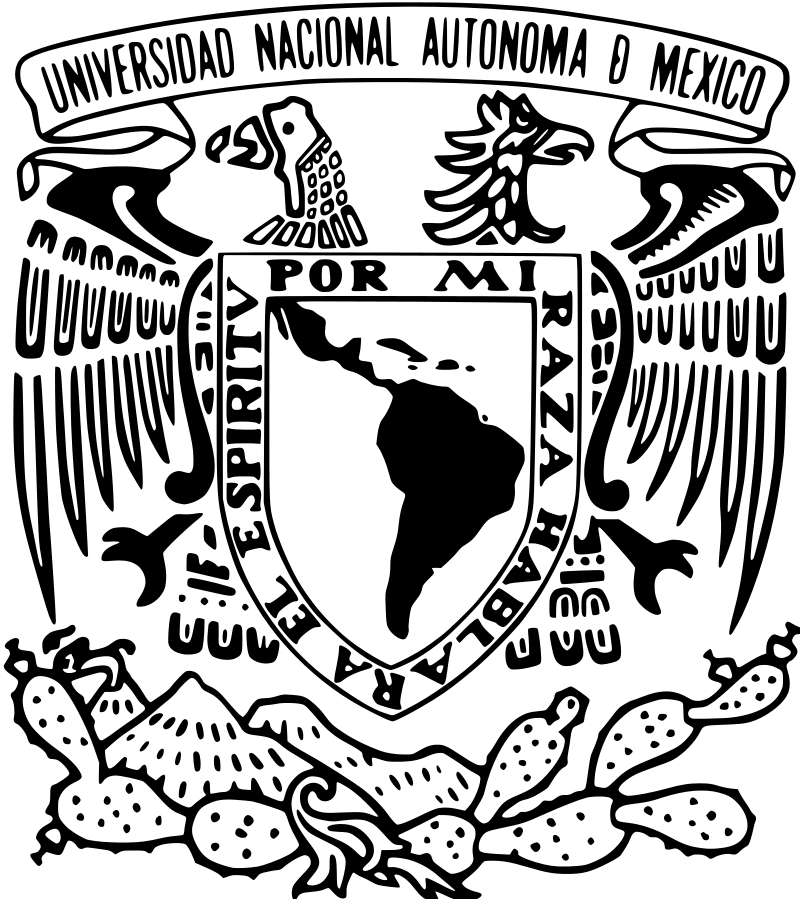
\includegraphics[width=4cm]{escudoUNAM_negro.png}
		% };

		\node[anchor=north east, inner sep=30] at (current page.north east) {
			
\includegraphics[width=3.5cm, height=4cm]{escudoFI_color.png}
		};
		% \node[anchor=north east, inner sep=30] at (current page.north east) {
		% 	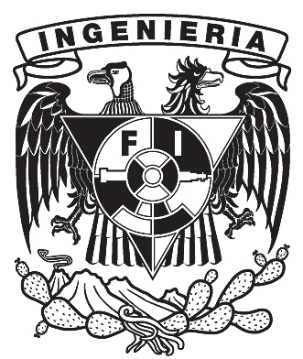
\includegraphics[width=4cm]{escudoFI_negro.png}
		% };
	\end{tikzpicture}

	\begin{center}
		\vspace*{3.5cm}

		\Large
		\textbf{UNIVERSIDAD NACIONAL AUTÓNOMA DE MÉXICO}\\
		\textbf{FACULTAD DE INGENIERÍA}\\
		\textbf{INGENIERÍA EN COMPUTACIÓN}\\

		\vspace*{1.5cm}
		\large
		\textbf{Laboratorio de Organización y Arquitectura de Computadoras}\\
		\large
		\vspace*{1cm}
		\textbf{Reporte - Construcción de Máquinas de Estados Usando Memorias}\\
		\vspace{1.5cm}
	\end{center}

	%grupo de la materia
	\large
	\textbf{INTEGRANTES EQUIPO 8:}
	\begin{itemize}
		\item Saldaña Navarrete Andrea - \textit{Grupo Teoria:} 2
		\item Tepal Briseño Hansel Yael - \textit{Grupo Teoria:} 1
		\item Ugartechea González Luis Antonio - \textit{Grupo Teoria:} 1
	\end{itemize}
	\vspace{2.5cm}

	\large
	%fecha de entrega
	\textbf{NOMBRE DELPROFESOR:} Ing. Diana Karen Pérez Pérez \\
	\textbf{GRUPO:} 06\\
	\textbf{SEMESTRE:} \underline{2027-1}\\
	\vspace{0.5cm}

	\begin{center}
		\textbf{FECHA DE ENTREGA:} 8 de octubre del 2026\\
	\end{center}
\end{titlepage}


\section*{Objetivo}

Familiarizar al alumno con la construcción de máquinas de estados mediante el uso de
memorias, aplicando el método de direccionamiento por trayectoria.

\section*{Introducción}

En el ámbito del diseño digital, el método de direccionamiento por trayectoria permite implementar cartas ASM almacenando el comportamiento lógico directamente en una memoria. Este tipo de direccionamiento guarda el estado siguiente y las salidas de cada estado en una localidad específica [\protect\hyperlink{1-diana-karen}{1}]. La porción de la memoria que se encarga de indicar cuál será el estado siguiente recibe el nombre de "liga", mientras que otra porción se destina a la parte de las salidas [\protect\hyperlink{1-diana-karen}{1}]. Para que el sistema determine la dirección de memoria exacta a la que debe acceder en cada pulso de reloj, se concatenan los bits de la liga del estado presente junto con las variables de entrada [\protect\hyperlink{1-diana-karen}{1}], [\protect\hyperlink{2-facultad-ingenieria}{2}].

Para poder construir el contenido de la tabla de memoria, es un requisito indispensable asignar previamente a cada estado de la carta ASM una codificación o representación binaria [\protect\hyperlink{1-diana-karen}{1}]. La cantidad mínima de bits requeridos depende del número total de estados de la máquina; por ejemplo, si se cuenta con 5 estados, se requieren por lo menos 3 bits para representarlos de manera binaria (ya que $2^3 = 8$ combinaciones posibles) [\protect\hyperlink{2-facultad-ingenieria}{2}]. Asimismo, la regla fundamental al momento de estructurar el contenido de memoria establece que, para cada estado, es necesario considerar todas las posibles combinaciones de las variables de entrada, aun cuando algunas de ellas no se utilicen de manera explícita en ese estado determinado [\protect\hyperlink{1-diana-karen}{1}].

Finalmente, el dimensionamiento y la organización de la memoria dependen directamente de la suma de variables. Si se diseña una carta ASM de 5 estados (3 bits de liga), 3 entradas y 4 salidas, la memoria requerirá un bus de direcciones de 6 bits (3 de liga + 3 de entrada) y palabras de 7 bits de longitud (3 de liga siguiente + 4 de salida). Esto da como resultado una organización de memoria de $2^6 \times 7$, es decir, de $64 \times 7$ bits [\protect\hyperlink{2-facultad-ingenieria}{2}].

\section*{Desarrollo}

\subsection*{1. Diseñe una carta ASM con las siguientes características:}

\begin{itemize}
    \item 5 estados
    \item 3 entradas
    \item 4 salidas
    \begin{itemize}
        \item 2 con lógica estándar
        \item 2 con lógica negada
    \end{itemize}
    \item Dada una entrada, colocar salidas condicionales en ambos caminos.
\end{itemize}

\begin{figure}[H]
    \centering
    \begin{tikzpicture}[
        state/.style={draw, rounded corners=2pt, fill=blue!10, minimum width=2.8cm, minimum height=1.2cm, align=center, font=\small},
        decision/.style={draw, diamond, aspect=2.1, fill=yellow!20, minimum width=1cm, minimum height=1cm, align=center, font=\small},
        output/.style={draw, rounded corners=15pt, fill=gray!15, minimum width=2cm, minimum height=1cm, align=center, font=\small},
        >={Stealth[length=2mm,width=2mm]}
    ]
        % Layout vertical: flujo principal de arriba hacia abajo
        \node[state, label={[anchor=south east, font=\small]north east:{000}}] (E1) at (0,0) {};
        \node[decision] (X1) at (0,-2) {\texttt{x}};
        \node[output] (U01) at (-4,-2) {$\overline{U_0}$};
        \node[output] (U11) at (4,-2) {$\overline{U_1}$};
        \node[decision] (Y1) at (-4,-4) {\texttt{y}};
        \node[output] (S01) at (-7,-2) {$S_0$};
        \node[state, label={[anchor=south east, font=\small]north east:{001}}] (E2) at (7,-4) {$S_0$};
        \node[output] (U02) at (-4,-6) {$\overline{U_0}$};
        \node[state, label={[anchor=south east, font=\small]north east:{011}}] (E4) at (-4,-8) {$\overline{U_1}$};
        \node[state, label={[anchor=south east, font=\small]north east:{010}}] (E3) at (7,-7) {$S_1$};
        \node[decision] (Z1) at (7,-9) {\texttt{z}};
        \node[output] (S02) at (4,-9) {$S_0$};
        \node[output] (U12) at (7,-11) {$\overline{U_1}$};
        \node[state, label={[anchor=south east, font=\small]north east:{100}}] (E5) at (7,-13) {$S_0 S_1 \overline{U_0} \overline{U_1}$};
        % Flechas principales con curva
        \draw[->] (E1) -- (X1);
        \draw[] (X1) -- node[above, font=\scriptsize] {1} (U01);
        \draw[] (X1) -- node[above, font=\scriptsize] {0} (U11);
        \draw[->] (U01) -- (Y1);
        \draw[] (Y1) -| node[above right, font=\scriptsize] {0} (S01);
        \draw[->] (S01) |- (E1);
        \draw[->] (U11) -| (E2);
        \draw[] (Y1) -- node[right, font=\scriptsize] {1} (U02);
        \draw[->] (U02) -- (E4);
        \draw[->] (E4.east) -- ++(1,0) |- (E2.west);
        \draw[->] (E2) -- (E3);
        \draw[->] (E3) -- (Z1);
        \draw[] (Z1) -- node[above, font=\scriptsize] {0} (S02);
        \draw[] (Z1) -- node[left, font=\scriptsize] {1} (U12);
        \draw[->] (S02) |- (E3);
        \draw[->] (U12) -- (E5);
        \draw[->] (E5.east) -- ++(1,0) |- (E1.east);
    \end{tikzpicture}
    \caption{Carta ASM para la máquina de estados del punto 1.}
\end{figure}

\begin{table}[H]
\renewcommand{\arraystretch}{1.2}
\begin{center}
    \begin{tabular}{|ccc|ccc|ccc|cccc|}
    \hline
    \rowcolor{black!80}
    \multicolumn{3}{|c|}{\textcolor{white}{\textbf{Estado Actual}}} & \multicolumn{3}{c|}{\textcolor{white}{\textbf{Entradas}}} & \multicolumn{3}{c|}{\textcolor{white}{\textbf{Estado Siguiente}}} & \multicolumn{4}{c|}{\textcolor{white}{\textbf{Salidas}}} \\
    \hline
    \rowcolor{black!80}
    \textcolor{white}{\textbf{$P_2(t)$}} & \textcolor{white}{\textbf{$P_1(t)$}} & \textcolor{white}{\textbf{$P_0(t)$}} & \textcolor{white}{\textbf{$X$}} & \textcolor{white}{\textbf{$Y$}} & \textcolor{white}{\textbf{$Z$}} & \textcolor{white}{\textbf{$L_2(t+1)$}} & \textcolor{white}{\textbf{$L_1(t+1)$}} & \textcolor{white}{\textbf{$L_0(t+1)$}} & \textcolor{white}{\textbf{$S_1$}} & \textcolor{white}{\textbf{$S_0$}} & \textcolor{white}{\textbf{$\overline{U_1}$}} & \textcolor{white}{\textbf{$\overline{U_0}$}} \\
    \hline
    0 & 0 & 0 & 0 & 0 & 0 & 0 & 0 & 1 & \cellcolor{ForestGreen!90}0 & \cellcolor{ForestGreen!90}0 & \cellcolor{ForestGreen!90}1 & \cellcolor{ForestGreen!90}1 \\
    0 & 0 & 0 & 0 & 0 & 1 & 0 & 0 & 1 & \cellcolor{ForestGreen!90}0 & \cellcolor{ForestGreen!90}0 & \cellcolor{ForestGreen!90}1 & \cellcolor{ForestGreen!90}1 \\
    0 & 0 & 0 & 0 & 1 & 0 & 0 & 0 & 1 & \cellcolor{ForestGreen!90}0 & \cellcolor{ForestGreen!90}0 & \cellcolor{ForestGreen!90}1 & \cellcolor{ForestGreen!90}1 \\
    0 & 0 & 0 & 0 & 1 & 1 & 0 & 0 & 1 & \cellcolor{ForestGreen!90}0 & \cellcolor{ForestGreen!90}0 & \cellcolor{ForestGreen!90}1 & \cellcolor{ForestGreen!90}1 \\
    0 & 0 & 0 & 1 & 0 & 0 & 0 & 0 & 0 & \cellcolor{ForestGreen!90}0 & \cellcolor{ForestGreen!90}0 & \cellcolor{ForestGreen!90}1 & \cellcolor{ForestGreen!90}1\\
    0 & 0 & 0 & 1 & 0 & 1 & 0 & 0 & 0 & \cellcolor{ForestGreen!90}0 & \cellcolor{ForestGreen!90}0 & \cellcolor{ForestGreen!90}1 & \cellcolor{ForestGreen!90}0\\
    0 & 0 & 0 & 1 & 1 & 0 & 0 & 1 & 1 & \cellcolor{ForestGreen!90}0 & \cellcolor{ForestGreen!90}0 & \cellcolor{ForestGreen!90}1 & \cellcolor{ForestGreen!90}0\\
    0 & 0 & 0 & 1 & 1 & 1 & 0 & 1 & 1 & \cellcolor{ForestGreen!90}0 & \cellcolor{ForestGreen!90}0 & \cellcolor{ForestGreen!90}1 & \cellcolor{ForestGreen!90}0\\
    \hline
    0 & 0 & 1 & 0 & 0 & 0 & 0 & 1 & 0 & \cellcolor{ForestGreen!90}0 & \cellcolor{ForestGreen!90}1 & \cellcolor{ForestGreen!90}1 & \cellcolor{ForestGreen!90}1 \\
    0 & 0 & 1 & 0 & 0 & 1 & 0 & 1 & 0 & \cellcolor{ForestGreen!90}0 & \cellcolor{ForestGreen!90}1 & \cellcolor{ForestGreen!90}1 & \cellcolor{ForestGreen!90}1 \\
    0 & 0 & 1 & 0 & 1 & 0 & 0 & 1 & 0 & \cellcolor{ForestGreen!90}0 & \cellcolor{ForestGreen!90}1 & \cellcolor{ForestGreen!90}1 & \cellcolor{ForestGreen!90}1 \\
    0 & 0 & 1 & 0 & 1 & 1 & 0 & 1 & 0 & \cellcolor{ForestGreen!90}0 & \cellcolor{ForestGreen!90}1 & \cellcolor{ForestGreen!90}1 & \cellcolor{ForestGreen!90}1 \\
    0 & 0 & 1 & 1 & 0 & 0 & 0 & 1 & 0 & \cellcolor{ForestGreen!90}0 & \cellcolor{ForestGreen!90}1 & \cellcolor{ForestGreen!90}1 & \cellcolor{ForestGreen!90}1 \\
    0 & 0 & 1 & 1 & 0 & 1 & 0 & 1 & 0 & \cellcolor{ForestGreen!90}0 & \cellcolor{ForestGreen!90}1 & \cellcolor{ForestGreen!90}1 & \cellcolor{ForestGreen!90}1 \\
    0 & 0 & 1 & 1 & 1 & 0 & 0 & 1 & 0 & \cellcolor{ForestGreen!90}0 & \cellcolor{ForestGreen!90}1 & \cellcolor{ForestGreen!90}1 & \cellcolor{ForestGreen!90}1 \\
    0 & 0 & 1 & 1 & 1 & 1 & 0 & 1 & 0 & \cellcolor{ForestGreen!90}0 & \cellcolor{ForestGreen!90}1 & \cellcolor{ForestGreen!90}1 & \cellcolor{ForestGreen!90}1 \\
    \hline
    0 & 1 & 0 & 0 & 0 & 0 & 0 & 1 & 0 & \cellcolor{ForestGreen!90}1 & \cellcolor{ForestGreen!90}1 & \cellcolor{ForestGreen!90}1 & \cellcolor{ForestGreen!90}1 \\
    0 & 1 & 0 & 0 & 0 & 1 & 1 & 0 & 0 & \cellcolor{ForestGreen!90}1 & \cellcolor{ForestGreen!90}0 & \cellcolor{ForestGreen!90}0 & \cellcolor{ForestGreen!90}1 \\
    0 & 1 & 0 & 0 & 1 & 0 & 0 & 1 & 0 & \cellcolor{ForestGreen!90}1 & \cellcolor{ForestGreen!90}1 & \cellcolor{ForestGreen!90}1 & \cellcolor{ForestGreen!90}1 \\
    0 & 1 & 0 & 0 & 1 & 1 & 1 & 0 & 0 & \cellcolor{ForestGreen!90}1 & \cellcolor{ForestGreen!90}0 & \cellcolor{ForestGreen!90}0 & \cellcolor{ForestGreen!90}1 \\
    0 & 1 & 0 & 1 & 0 & 0 & 0 & 1 & 0 & \cellcolor{ForestGreen!90}1 & \cellcolor{ForestGreen!90}1 & \cellcolor{ForestGreen!90}1 & \cellcolor{ForestGreen!90}1 \\
    0 & 1 & 0 & 1 & 0 & 1 & 1 & 0 & 0 & \cellcolor{ForestGreen!90}1 & \cellcolor{ForestGreen!90}0 & \cellcolor{ForestGreen!90}0 & \cellcolor{ForestGreen!90}1 \\
    0 & 1 & 0 & 1 & 1 & 0 & 0 & 1 & 0 & \cellcolor{ForestGreen!90}1 & \cellcolor{ForestGreen!90}1 & \cellcolor{ForestGreen!90}1 & \cellcolor{ForestGreen!90}1 \\
    0 & 1 & 0 & 1 & 1 & 1 & 1 & 0 & 0 & \cellcolor{ForestGreen!90}1 & \cellcolor{ForestGreen!90}0 & \cellcolor{ForestGreen!90}0 & \cellcolor{ForestGreen!90}1 \\
    \hline
    0 & 1 & 1 & 0 & 0 & 0 & 0 & 0 & 1 & \cellcolor{ForestGreen!90}0 & \cellcolor{ForestGreen!90}0 & \cellcolor{ForestGreen!90}0 & \cellcolor{ForestGreen!90}1 \\
    0 & 1 & 1 & 0 & 0 & 1 & 0 & 0 & 1 & \cellcolor{ForestGreen!90}0 & \cellcolor{ForestGreen!90}0 & \cellcolor{ForestGreen!90}0 & \cellcolor{ForestGreen!90}1 \\
    0 & 1 & 1 & 0 & 1 & 0 & 0 & 0 & 1 & \cellcolor{ForestGreen!90}0 & \cellcolor{ForestGreen!90}0 & \cellcolor{ForestGreen!90}0 & \cellcolor{ForestGreen!90}1 \\
    0 & 1 & 1 & 0 & 1 & 1 & 0 & 0 & 1 & \cellcolor{ForestGreen!90}0 & \cellcolor{ForestGreen!90}0 & \cellcolor{ForestGreen!90}0 & \cellcolor{ForestGreen!90}1 \\
    0 & 1 & 1 & 1 & 0 & 0 & 0 & 0 & 1 & \cellcolor{ForestGreen!90}0 & \cellcolor{ForestGreen!90}0 & \cellcolor{ForestGreen!90}0 & \cellcolor{ForestGreen!90}1 \\
    0 & 1 & 1 & 1 & 0 & 1 & 0 & 0 & 1 & \cellcolor{ForestGreen!90}0 & \cellcolor{ForestGreen!90}0 & \cellcolor{ForestGreen!90}0 & \cellcolor{ForestGreen!90}1 \\
    0 & 1 & 1 & 1 & 1 & 0 & 0 & 0 & 1 & \cellcolor{ForestGreen!90}0 & \cellcolor{ForestGreen!90}0 & \cellcolor{ForestGreen!90}0 & \cellcolor{ForestGreen!90}1 \\
    0 & 1 & 1 & 1 & 1 & 1 & 0 & 0 & 1 & \cellcolor{ForestGreen!90}0 & \cellcolor{ForestGreen!90}0 & \cellcolor{ForestGreen!90}0 & \cellcolor{ForestGreen!90}1 \\
    \hline
    \end{tabular}
\end{center}
\caption{Tabla de transiciones y salidas de la máquina de estados.}
\label{tab:tabla_transiciones_estados_salidas_1}
\end{table}

\begin{table}[H]
\renewcommand{\arraystretch}{1.2}
\begin{center}
    \begin{tabular}{|ccc|ccc|ccc|cccc|}
    \hline
    \rowcolor{black!80}
    \multicolumn{3}{|c|}{\textcolor{white}{\textbf{Estado Actual}}} & \multicolumn{3}{c|}{\textcolor{white}{\textbf{Entradas}}} & \multicolumn{3}{c|}{\textcolor{white}{\textbf{Estado Siguiente}}} & \multicolumn{4}{c|}{\textcolor{white}{\textbf{Salidas}}} \\
    \hline
    \rowcolor{black!80}
    \textcolor{white}{\textbf{$P_2(t)$}} & \textcolor{white}{\textbf{$P_1(t)$}} & \textcolor{white}{\textbf{$P_0(t)$}} & \textcolor{white}{\textbf{$X$}} & \textcolor{white}{\textbf{$Y$}} & \textcolor{white}{\textbf{$Z$}} & \textcolor{white}{\textbf{$L_2(t+1)$}} & \textcolor{white}{\textbf{$L_1(t+1)$}} & \textcolor{white}{\textbf{$L_0(t+1)$}} & \textcolor{white}{\textbf{$S_1$}} & \textcolor{white}{\textbf{$S_0$}} & \textcolor{white}{\textbf{$\overline{U_1}$}} & \textcolor{white}{\textbf{$\overline{U_0}$}} \\
    \hline
    1 & 0 & 0 & 0 & 0 & 0 & 0 & 0 & 0 & \cellcolor{ForestGreen!90}1 & \cellcolor{ForestGreen!90}1 & \cellcolor{ForestGreen!90}0 & \cellcolor{ForestGreen!90}0 \\
    1 & 0 & 0 & 0 & 0 & 1 & 0 & 0 & 0 & \cellcolor{ForestGreen!90}1 & \cellcolor{ForestGreen!90}1 & \cellcolor{ForestGreen!90}0 & \cellcolor{ForestGreen!90}0 \\
    1 & 0 & 0 & 0 & 1 & 0 & 0 & 0 & 0 & \cellcolor{ForestGreen!90}1 & \cellcolor{ForestGreen!90}1 & \cellcolor{ForestGreen!90}0 & \cellcolor{ForestGreen!90}0 \\
    1 & 0 & 0 & 0 & 1 & 1 & 0 & 0 & 0 & \cellcolor{ForestGreen!90}1 & \cellcolor{ForestGreen!90}1 & \cellcolor{ForestGreen!90}0 & \cellcolor{ForestGreen!90}0 \\
    1 & 0 & 0 & 1 & 0 & 0 & 0 & 0 & 0 & \cellcolor{ForestGreen!90}1 & \cellcolor{ForestGreen!90}1 & \cellcolor{ForestGreen!90}0 & \cellcolor{ForestGreen!90}0 \\
    1 & 0 & 0 & 1 & 0 & 1 & 0 & 0 & 0 & \cellcolor{ForestGreen!90}1 & \cellcolor{ForestGreen!90}1 & \cellcolor{ForestGreen!90}0 & \cellcolor{ForestGreen!90}0 \\
    1 & 0 & 0 & 1 & 1 & 0 & 0 & 0 & 0 & \cellcolor{ForestGreen!90}1 & \cellcolor{ForestGreen!90}1 & \cellcolor{ForestGreen!90}0 & \cellcolor{ForestGreen!90}0 \\
    1 & 0 & 0 & 1 & 1 & 1 & 0 & 0 & 0 & \cellcolor{ForestGreen!90}1 & \cellcolor{ForestGreen!90}1 & \cellcolor{ForestGreen!90}0 & \cellcolor{ForestGreen!90}0 \\
    \hline
    1 & 0 & 1 & 0 & 0 & 0 & 0 & 0 & 0 & \cellcolor{ForestGreen!90}0 & \cellcolor{ForestGreen!90}0 & \cellcolor{ForestGreen!90}0 & \cellcolor{ForestGreen!90}0 \\
    1 & 0 & 1 & 0 & 0 & 1 & 0 & 0 & 0 & \cellcolor{ForestGreen!90}0 & \cellcolor{ForestGreen!90}0 & \cellcolor{ForestGreen!90}0 & \cellcolor{ForestGreen!90}0 \\
    1 & 0 & 1 & 0 & 1 & 0 & 0 & 0 & 0 & \cellcolor{ForestGreen!90}0 & \cellcolor{ForestGreen!90}0 & \cellcolor{ForestGreen!90}0 & \cellcolor{ForestGreen!90}0 \\
    1 & 0 & 1 & 0 & 1 & 1 & 0 & 0 & 0 & \cellcolor{ForestGreen!90}0 & \cellcolor{ForestGreen!90}0 & \cellcolor{ForestGreen!90}0 & \cellcolor{ForestGreen!90}0 \\
    1 & 0 & 1 & 1 & 0 & 0 & 0 & 0 & 0 & \cellcolor{ForestGreen!90}0 & \cellcolor{ForestGreen!90}0 & \cellcolor{ForestGreen!90}0 & \cellcolor{ForestGreen!90}0 \\
    1 & 0 & 1 & 1 & 0 & 1 & 0 & 0 & 0 & \cellcolor{ForestGreen!90}0 & \cellcolor{ForestGreen!90}0 & \cellcolor{ForestGreen!90}0 & \cellcolor{ForestGreen!90}0 \\
    1 & 0 & 1 & 1 & 1 & 0 & 0 & 0 & 0 & \cellcolor{ForestGreen!90}0 & \cellcolor{ForestGreen!90}0 & \cellcolor{ForestGreen!90}0 & \cellcolor{ForestGreen!90}0 \\
    1 & 0 & 1 & 1 & 1 & 1 & 0 & 0 & 0 & \cellcolor{ForestGreen!90}0 & \cellcolor{ForestGreen!90}0 & \cellcolor{ForestGreen!90}0 & \cellcolor{ForestGreen!90}0 \\
    \hline
    1 & 1 & 0 & 0 & 0 & 0 & 0 & 0 & 0 & \cellcolor{ForestGreen!90}0 & \cellcolor{ForestGreen!90}0 & \cellcolor{ForestGreen!90}0 & \cellcolor{ForestGreen!90}0 \\
    1 & 1 & 0 & 0 & 0 & 1 & 0 & 0 & 0 & \cellcolor{ForestGreen!90}0 & \cellcolor{ForestGreen!90}0 & \cellcolor{ForestGreen!90}0 & \cellcolor{ForestGreen!90}0 \\
    1 & 1 & 0 & 0 & 1 & 0 & 0 & 0 & 0 & \cellcolor{ForestGreen!90}0 & \cellcolor{ForestGreen!90}0 & \cellcolor{ForestGreen!90}0 & \cellcolor{ForestGreen!90}0 \\
    1 & 1 & 0 & 0 & 1 & 1 & 0 & 0 & 0 & \cellcolor{ForestGreen!90}0 & \cellcolor{ForestGreen!90}0 & \cellcolor{ForestGreen!90}0 & \cellcolor{ForestGreen!90}0 \\
    1 & 1 & 0 & 1 & 0 & 0 & 0 & 0 & 0 & \cellcolor{ForestGreen!90}0 & \cellcolor{ForestGreen!90}0 & \cellcolor{ForestGreen!90}0 & \cellcolor{ForestGreen!90}0 \\
    1 & 1 & 0 & 1 & 0 & 1 & 0 & 0 & 0 & \cellcolor{ForestGreen!90}0 & \cellcolor{ForestGreen!90}0 & \cellcolor{ForestGreen!90}0 & \cellcolor{ForestGreen!90}0 \\
    1 & 1 & 0 & 1 & 1 & 0 & 0 & 0 & 0 & \cellcolor{ForestGreen!90}0 & \cellcolor{ForestGreen!90}0 & \cellcolor{ForestGreen!90}0 & \cellcolor{ForestGreen!90}0 \\
    1 & 1 & 0 & 1 & 1 & 1 & 0 & 0 & 0 & \cellcolor{ForestGreen!90}0 & \cellcolor{ForestGreen!90}0 & \cellcolor{ForestGreen!90}0 & \cellcolor{ForestGreen!90}0 \\
    \hline
    1 & 1 & 1 & 0 & 0 & 0 & 0 & 0 & 0 & \cellcolor{ForestGreen!90}0 & \cellcolor{ForestGreen!90}0 & \cellcolor{ForestGreen!90}0 & \cellcolor{ForestGreen!90}0 \\
    1 & 1 & 1 & 0 & 0 & 1 & 0 & 0 & 0 & \cellcolor{ForestGreen!90}0 & \cellcolor{ForestGreen!90}0 & \cellcolor{ForestGreen!90}0 & \cellcolor{ForestGreen!90}0 \\
    1 & 1 & 1 & 0 & 1 & 0 & 0 & 0 & 0 & \cellcolor{ForestGreen!90}0 & \cellcolor{ForestGreen!90}0 & \cellcolor{ForestGreen!90}0 & \cellcolor{ForestGreen!90}0 \\
    1 & 1 & 1 & 0 & 1 & 1 & 0 & 0 & 0 & \cellcolor{ForestGreen!90}0 & \cellcolor{ForestGreen!90}0 & \cellcolor{ForestGreen!90}0 & \cellcolor{ForestGreen!90}0 \\
    1 & 1 & 1 & 1 & 0 & 0 & 0 & 0 & 0 & \cellcolor{ForestGreen!90}0 & \cellcolor{ForestGreen!90}0 & \cellcolor{ForestGreen!90}0 & \cellcolor{ForestGreen!90}0 \\
    1 & 1 & 1 & 1 & 0 & 1 & 0 & 0 & 0 & \cellcolor{ForestGreen!90}0 & \cellcolor{ForestGreen!90}0 & \cellcolor{ForestGreen!90}0 & \cellcolor{ForestGreen!90}0 \\
    1 & 1 & 1 & 1 & 1 & 0 & 0 & 0 & 0 & \cellcolor{ForestGreen!90}0 & \cellcolor{ForestGreen!90}0 & \cellcolor{ForestGreen!90}0 & \cellcolor{ForestGreen!90}0 \\
    1 & 1 & 1 & 1 & 1 & 1 & 0 & 0 & 0 & \cellcolor{ForestGreen!90}0 & \cellcolor{ForestGreen!90}0 & \cellcolor{ForestGreen!90}0 & \cellcolor{ForestGreen!90}0 \\
    \hline
    \end{tabular}
\end{center}
\caption{Tabla de transiciones y salidas de la máquina de estados.}
\label{tab:tabla_transiciones_estados_salidas_2}
\end{table}

\subsection*{2. Encuentre el tamaño de la memoria necesaria y el contenido de memoria utilizando  el direccionamiento por trayectoria.}

Recuerde que antes de construir la tabla se debe asignar a cada estado de la carta ASM una representación binaria. Así mismo, recuerde que para cada estado es necesario considerar todas las posibles combinaciones de las variables de entrada, aun cuando algunas de ellas no se utilicen en determinado estado. Para esto se utiliza:

\textbf{Tamaño de memoria estandar:}

\[2^n \cdot (m)\]

En donde:
\begin{itemize}
    \item $n$ = Número de bits de estado + Número de entradas
    \item $m$ = Número de bits liga + Número de salidas
\end{itemize}

En este caso tenemos 3 bits de estado y 3 bits de entrada, por lo que $n = 6$. Además, tenemos 3 bits de liga y 4 bits de salida, por lo que $m = 7$. Por lo tanto, el tamaño de memoria necesario es:

\begin{tcolorbox}[colback=gray!20,colframe=LimeGreen!75!black]
\[2^6 \cdot 7 = 448 \text{ bits}\]
\end{tcolorbox}

\textbf{Tamaño de memoria óptimo:}

\[\texttt{Número de estados} \cdot 2^{\texttt{Número de estados}} \cdot (log_2(\texttt{Número de estados})) + \texttt{Número de salidas}\]

\begin{tcolorbox}[colback=gray!20,colframe=LimeGreen!75!black]
\[5\cdot 2^3 \cdot (log_2(5)) + 4 = 96.8771238 \text{ bits}\]
\end{tcolorbox}

\subsection*{3. Implementación de direccionamiento por trayectoria en Quartus.}

La implementación se realizó en Quartus Prime 18.1 Lite, seleccionando la familia MAX 10 y el dispositivo 10M50DCF484C7G. El archivo \texttt{practica\_3.bdf} se utilizó como entidad de nivel superior; en él se conectaron los bloques que forman la ruta de datos de la máquina: el divisor de frecuencia, el registro de estado, el concatenador de dirección, la memoria y el divisor de datos.

El funcionamiento es síncrono. El divisor de frecuencia genera el reloj lento a partir de la señal de la FPGA y el registro conserva el estado presente. Este estado se concatena con las tres entradas externas para formar una dirección de seis bits. La memoria entrega una palabra de siete bits, formada por tres bits de liga y cuatro bits de salida. Finalmente, el divisor de datos separa ambos campos: la liga se conecta a la entrada del registro y las salidas se conectan a los LED de la tarjeta.

La dirección de memoria se construye mediante concatenación directa. La expresión \texttt{entradaB \& entradaA} coloca primero el estado presente y después las entradas, por lo que cada combinación de estado y entradas selecciona una localidad distinta de la ROM.

\begin{lstlisting}[style=vhdl, caption={Construcción de la dirección de memoria mediante el estado presente y las entradas.}, label={lst:concatenador_datos}]
entity concatenador_datos is
    Port ( entradaA : in  STD_LOGIC_VECTOR(2 downto 0);
           entradaB : in  STD_LOGIC_VECTOR(2 downto 0);
           salida   : out STD_LOGIC_VECTOR(5 downto 0) );
end concatenador_datos;

architecture Behavioral of concatenador_datos is
begin
    process (entradaA, entradaB)
    begin
        salida <= entradaB & entradaA;
    end process;
end Behavioral;
\end{lstlisting}

El contenido de la carta ASM se almacenó en una ROM de 64 localidades de siete bits. Cada entrada de la tabla se escribe como la concatenación de la liga del estado siguiente con las cuatro salidas. Por ejemplo, las primeras ocho localidades corresponden al estado presente `000` y contemplan las ocho combinaciones posibles de las tres entradas.

\begin{lstlisting}[style=vhdl, caption={Declaración de la ROM y ejemplo de sus palabras de control.}, label={lst:memory_rom}]
type rom_type is array (0 to 63) of std_logic_vector(6 downto 0);
signal internal_mem : rom_type := (
    0 => "001" & "0011", -- Estado 000, entradas 000
    1 => "001" & "0011", -- Estado 000, entradas 001
    2 => "001" & "0011", -- Estado 000, entradas 010
    3 => "001" & "0011", -- Estado 000, entradas 011
    4 => "000" & "0011", -- Estado 000, entradas 100
    5 => "000" & "0010", -- Estado 000, entradas 101
    6 => "011" & "0010", -- Estado 000, entradas 110
    7 => "011" & "0010", -- Estado 000, entradas 111
    others => "000" & "0000"
);

data <= internal_mem(conv_integer(unsigned(dir)));
\end{lstlisting}

La palabra obtenida de la memoria se divide en dos campos. Los tres bits más significativos representan la liga, es decir, el estado que será cargado en el siguiente flanco de reloj; los cuatro bits menos significativos representan las salidas actuales.

\begin{lstlisting}[style=vhdl, caption={Separación de la liga y las salidas de la palabra de memoria.}, label={lst:divisor_datos}]
process (entrada)
begin
    liga    <= entrada(6 downto 4);
    salidas <= entrada(3 downto 0);
end process;
\end{lstlisting}

El registro de estado carga la liga únicamente en el flanco ascendente del reloj dividido. El reinicio es activo en bajo, por lo que al activar `RESET` el estado se fuerza a `000`. Esta señalización coincide con las conexiones del diagrama esquemático y permite observar la secuencia de estados en la FPGA.

\begin{lstlisting}[style=vhdl, caption={Registro del estado presente con reinicio activo en bajo.}, label={lst:register2}]
process (CLK, RESET)
begin
    if RESET = '0' then
        internal_value <= B"000";
    elsif rising_edge (CLK) then
        internal_value <= DATA_IN;
    end if;
end process;
\end{lstlisting}

Después de agregar los archivos VHDL y el archivo de diagrama al proyecto, se asignaron los pines de reloj, reinicio, entradas y salidas en el archivo de configuración de Quartus.

\subsection*{4. Demuestre el correcto funcionamiento de su carta ASM cargando su código por equipos a su FPGA y mostrándola a la profesora en el laboratorio.}

% \begin{tcolorbox}[colback=gray!20,colframe=LimeGreen!75!black]
%     Los incisos 3 y 4 se resuelven de manera conjunta en la siguiente tabla de verdad general y más completa de la máquina de estados:

%     \begin{table}[H]
%     \renewcommand{\arraystretch}{1.2}
%     \begin{center}
%         \begin{tabular}{|cc|cc|cc|cc|}
%         \hline
%         \rowcolor{black!80}
%         \multicolumn{2}{|c|}{\textcolor{white}{\textbf{Estado Actual}}} & \multicolumn{2}{c|}{\textcolor{white}{\textbf{Entradas}}} & \multicolumn{2}{c|}{\textcolor{white}{\textbf{Estado Siguiente}}} & \multicolumn{2}{c|}{\textcolor{white}{\textbf{Salidas}}} \\
%         \hline
%         \rowcolor{black!80}
%         \textcolor{white}{\textbf{$E_1(t)$}} & \textcolor{white}{\textbf{$E_0(t)$}} & \textcolor{white}{\textbf{$X$}} & \textcolor{white}{\textbf{$Y$}} & \textcolor{white}{\textbf{$Q_1(t+1)$}} & \textcolor{white}{\textbf{$Q_0(t+1)$}} & \textcolor{white}{\textbf{$S_1$}} & \textcolor{white}{\textbf{$S_0$}} \\
%         \hline
%         0 & 0 & 0 & 0 & 0 & 0 & \cellcolor{ForestGreen!90}1 & \cellcolor{ForestGreen!90}0 \\
%         0 & 0 & 0 & 1 & 0 & 0 & \cellcolor{ForestGreen!90}1 & \cellcolor{ForestGreen!90}0 \\
%         0 & 0 & 1 & 0 & 0 & 0 & \cellcolor{ForestGreen!90}1 & \cellcolor{ForestGreen!90}0 \\
%         0 & 0 & 1 & 1 & 0 & 1 & \cellcolor{ForestGreen!90}1 & \cellcolor{ForestGreen!90}0 \\
%         \hline
%         0 & 1 & 0 & 0 & 0 & 1 & \cellcolor{ForestGreen!90}0 & \cellcolor{ForestGreen!90}1 \\
%         0 & 1 & 0 & 1 & 0 & 1 & \cellcolor{ForestGreen!90}0 & \cellcolor{ForestGreen!90}1 \\
%         0 & 1 & 1 & 0 & 0 & 1 & \cellcolor{ForestGreen!90}0 & \cellcolor{ForestGreen!90}1 \\
%         0 & 1 & 1 & 1 & 1 & 0 & \cellcolor{ForestGreen!90}0 & \cellcolor{ForestGreen!90}1 \\
%         \hline
%         1 & 0 & 0 & 0 & 1 & 1 & \cellcolor{ForestGreen!90}0 & \cellcolor{ForestGreen!90}0 \\
%         1 & 0 & 0 & 1 & 1 & 1 & \cellcolor{ForestGreen!90}0 & \cellcolor{ForestGreen!90}0 \\
%         1 & 0 & 1 & 0 & 1 & 1 & \cellcolor{ForestGreen!90}0 & \cellcolor{ForestGreen!90}0 \\
%         1 & 0 & 1 & 1 & 1 & 1 & \cellcolor{ForestGreen!90}0 & \cellcolor{ForestGreen!90}0 \\
%         \hline
%         1 & 1 & 0 & 0 & 0 & 0 & \cellcolor{ForestGreen!90}1 & \cellcolor{ForestGreen!90}1 \\
%         1 & 1 & 0 & 1 & 0 & 0 & \cellcolor{ForestGreen!90}1 & \cellcolor{ForestGreen!90}1 \\
%         1 & 1 & 1 & 0 & 0 & 0 & \cellcolor{ForestGreen!90}1 & \cellcolor{ForestGreen!90}1 \\
%         1 & 1 & 1 & 1 & 0 & 0 & \cellcolor{ForestGreen!90}1 & \cellcolor{ForestGreen!90}1 \\
%         \hline
%         \end{tabular}
%     \end{center}
%     \caption{Tabla de transiciones y salidas de la máquina de estados.}
%     \label{tab:tabla_transiciones_estados_salidas}
%     \end{table}
% \end{tcolorbox}

\subsection*{5. Simule su diseño para probar su funcionamiento. Recuerden que en sus simulaciones debe aparecer el contenido de la memoria además del estado presente.}


\section*{Análisis de Resultados}



\subsection*{Discusión de Resultados}


\section*{Conclusiones}

\subsection*{Andrea Saldaña Navarrete - 320206384}



\subsection*{Hansel Yael Tepal Briseño - 320078282}



\subsection*{Luis Antonio Ugartechea González - 320223822}


\newpage
\section{Bibliografía}

% En formato IEEE

\begin{biblio}
	\hypertarget{1-diana-karen}{}
	\item D. K. Pérez Pérez, ``Reporte Construcción de Máquinas de Estados Usando Memorias'', Laboratorio de Organización y Arquitectura de Computadoras, Facultad de Ingeniería, Universidad Nacional Autónoma de México, Semestre 2027-1, 2026.
	\hypertarget{2-facultad-ingenieria}{}
	\item Facultad de Ingeniería, ``Capítulo III: Construcción de máquinas de estados usando memorias'', Apuntes de Arquitectura de Computadoras, Universidad Nacional Autónoma de México (UNAM). [En línea]. Disponible en: \url{https://biorobotics.fi-p.unam.mx/wp-content/uploads/Courses/arquitectura_de_computadoras/2021-1/lecciones/Leccion_3_arquitectura_de_computadoras_2021_1.pdf}
	% \hypertarget{3-savage}{}
	\item J. Savage, \textit{Diseño de Microprocesadores}, Facultad de Ingeniería, Universidad Nacional Autónoma de México (UNAM). [En línea]. Disponible en: \url{http://profesores.fi-b.unam.mx/luist/archivos/MicroprocesadoresSavage.pdf}
\end{biblio}

\end{document}
